% ALGUNOS PAQUETES REQUERIDOS (EN UBUNTU): %
% ========================================
% %
% texlive-latex-base %
% texlive-latex-recommended %
% texlive-fonts-recommended %
% texlive-latex-extra %
% texlive-lang-spanish (en ubuntu 13.10) %
% ******************************************************** %

\documentclass[a4paper]{article}
\usepackage[spanish]{babel}
\usepackage[utf8]{inputenc}
\usepackage{fancyhdr}
\usepackage[pdftex]{graphicx}
\usepackage{sidecap}
\usepackage{caption}
\usepackage{subcaption}
\usepackage{booktabs}
\usepackage{makeidx}
\usepackage{float}
\usepackage{amsmath, amsthm, amssymb}
\usepackage{amsfonts}
\usepackage{sectsty}
\usepackage{wrapfig}
\usepackage{listings}
\usepackage{pgfplots}
\usepackage{enumitem}
\usepackage[hidelinks]{hyperref}
\usepackage{listings}
\usepackage{listingsutf8}
\usepackage{multirow}

\linespread{factor}

\definecolor{mygreen}{rgb}{0,0.6,0}
\definecolor{mygray}{rgb}{0.5,0.5,0.5}
\pgfplotsset{compat=1.3}
\setlist[enumerate]{label*=\arabic*.}
\lstset{
	inputencoding=utf8/latin1,
	language=C++,
	basicstyle=\ttfamily,
	keywordstyle=\bfseries\color{blue},
	stringstyle=\color{red}\ttfamily,
	commentstyle=\color{mygreen}\ttfamily,
	morecomment=[l][\color{magenta}]{\#},
	numbers=left,
	numberstyle=\color{mygray}
}

\usepackage{color} % para snipets de codigo coloreados
\usepackage{fancybox}  % para el sbox de los snipets de codigo

\definecolor{litegrey}{gray}{0.94}

% \newenvironment{sidebar}{%
% 	\begin{Sbox}\begin{minipage}{.85\textwidth}}%
% 	{\end{minipage}\end{Sbox}%
% 		\begin{center}\setlength{\fboxsep}{6pt}%
% 		\shadowbox{\TheSbox}\end{center}}
% \newenvironment{warning}{%
% 	\begin{Sbox}\begin{minipage}{.85\textwidth}\sffamily\lite\small\RaggedRight}%
% 	{\end{minipage}\end{Sbox}%
% 		\begin{center}\setlength{\fboxsep}{6pt}%
% 		\colorbox{litegrey}{\TheSbox}\end{center}}

\newenvironment{codesnippet}{%
	\begin{Sbox}\begin{minipage}{\textwidth}\sffamily\small}%
	{\end{minipage}\end{Sbox}%
		\begin{center}%
		\vspace{-0.4cm}\colorbox{litegrey}{\TheSbox}\end{center}\vspace{0.3cm}}



\usepackage{fancyhdr}
\pagestyle{fancy}
%\renewcommand{\chaptermark}[1]{\markboth{#1}{}}
\renewcommand{\sectionmark}[1]{\markright{\thesection\ - #1}}
\fancyhf{}
\fancyhead[LO]{Sección \rightmark} % \thesection\
\fancyfoot[LO]{\small{Franco Frizzo, Iván Pondal, Maximiliano León Paz}}
\fancyfoot[RO]{\thepage}
\renewcommand{\headrulewidth}{0.5pt}
\renewcommand{\footrulewidth}{0.5pt}
%\setlength{\hoffset}{-0.8in}
\setlength{\textwidth}{16cm}
\setlength{\hoffset}{-1.1cm}
\setlength{\headsep}{0.5cm}
\setlength{\textheight}{25cm}
\setlength{\voffset}{-0.7in}
\setlength{\headwidth}{\textwidth}
\setlength{\headheight}{13.1pt}
\renewcommand{\baselinestretch}{1.1} % line spacing

\usepackage{caratula}

\newcommand{\ord}{\ensuremath{\operatorname{O}}}
\newcommand{\nat}{\ensuremath{\mathbb{N}}}

%\lstset{
%    language=C++,
%    basicstyle=\ttfamily,
%    keywordstyle=\color{blue}\ttfamily,
%    stringstyle=\color{red}\ttfamily,
%    commentstyle=\color{ForestGreen}\ttfamily,
%    morecomment=[l][\color{magenta}]{\#}
%}

\begin{document}
\materia{Sistemas Operativos}
\submateria{Primer Cuatrimestre de 2016}
\titulo{Trabajo Práctico 1}
\subtitulo{Scheduling}
\integrante{Franco Frizzo}{013/14}{francofrizzo@gmail.com}
\integrante{Iván Pondal}{078/14}{ivan.pondal@gmail.com}
\integrante{Maximiliano León Paz}{251/14}{m4xileon@gmail.com}

\maketitle
% no footer on the first page
\thispagestyle{empty}

\newpage
\tableofcontents

\newpage
\section{Ejercicio 1}

Para la resolución de este ejercicio se requería generar \emph{n} tareas
bloqueantes con una duración aleatoria de valor $bmin \leq t \leq bmax$. La forma de
lograr esto fue mediante un ciclo que realiza \emph{n} llamados bloqueantes cuya
duración está dictaminada por el siguiente código:

\begin{center}
	\texttt{t = rand() \% (bmax - bmin + 1) + bmin;}
\end{center}

Se utiliza la función \texttt{rand()} habiendo previamente cargado una semilla.
Esto genera un valor $0 \leq r \leq RAND\_MAX$. Para que quede dentro de los
límites definidos con anterioridad, se toma el módulo correspondiente de
\emph{r} sumándole luego \emph{bmin}.

\begin{figure}[ht]
	\begin{center}
		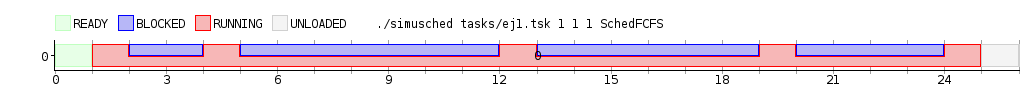
\includegraphics[width=1\columnwidth]{imagenes/ej1.png}
		\caption{\texttt{TaskConsola} corriendo con $n = 4$, $bmin = 2$ y $bmax
		= 7$.}
	\end{center}
\end{figure}


\section{Ejercicio 2}

Se pedía escribir un lote de tareas que simulara la utilización de una
computadora para resolver un problema de Data Mining y, simultáneamente, como
servidor para tres clientes que realizan tareas bloqueantes. Esto se realizó
utilizando una tarea \texttt{TaskCPU} con una duración de 500, y tres tareas de
tipo \texttt{TaskIORandom}. Esta tarea recibe tres parámetros ($ms\_cpu$, $bmin$
y $bmax$) y realiza, en tiempo $ms\_cpu$, una llamada bloqueante con una duración
aleatoria entre $bmin$ y $bmax$. En los tres casos se consideró $bmin = 1$ y
$bim = 4$, mientras que para $ms\_cpu$ se tomaron los valores $10$, $20$ y $30$.

A continuación se exponen los gráficos obtenidos, considerando un costo para el cambio de contexto de 5 ciclos de CPU.

\begin{figure}[H]
    \begin{center}
        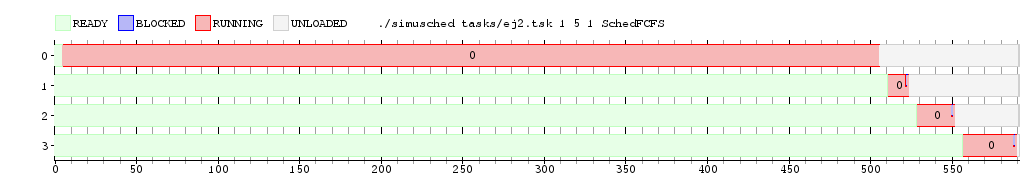
\includegraphics[width=1\columnwidth]{imagenes/ej2_1.png}
        \caption{Lote \texttt{ej2} corriendo en 1 núcleo}
    \end{center}
\end{figure}

\begin{figure}[H]
    \begin{center}
        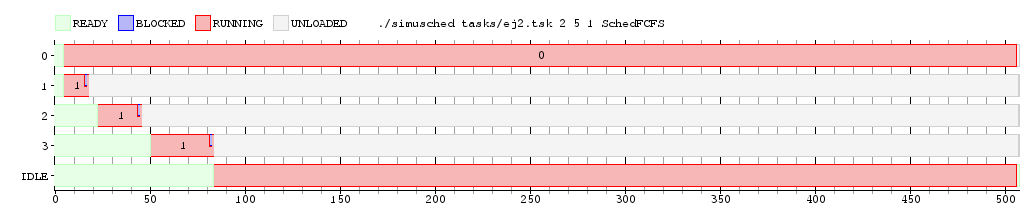
\includegraphics[width=1\columnwidth]{imagenes/ej2_2.png}
        \caption{Lote \texttt{ej2} corriendo en 2 núcleos}
    \end{center}
\end{figure}

\begin{figure}[H]
    \begin{center}
        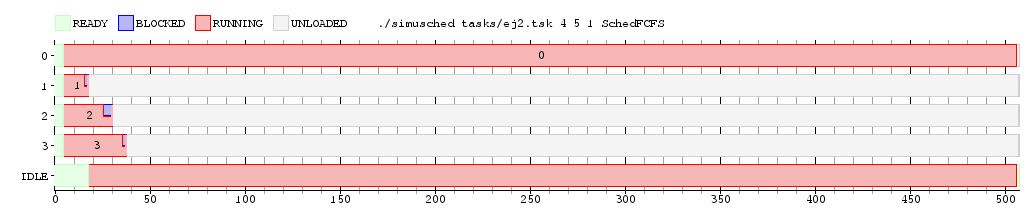
\includegraphics[width=1\columnwidth]{imagenes/ej2_3.png}
        \caption{Lote \texttt{ej2} corriendo en 4 núcleos}
    \end{center}
\end{figure}

Calculando, en los tres escenarios, la \emph{latencia} de cada tarea, se obtiene:

\begin{table}[H]
    \begin{center}
        \begin{tabular}{|c|c|c|c|c|}
            \hline
            & \multicolumn{4}{c|}{\textbf{Latencia}} \\ \hline
            \textbf{Cant. núcleos} & \texttt{TaskCPU} & \texttt{TaskIORandom (1)} & \texttt{TaskIORandom (2)} & \texttt{TaskIORandom (3)} \\ \hline
            1 & 5 & 511 & 531 & 561 \\
            2 & 5 & 5 & 24 & 53 \\
            4 & 5 & 5 & 5 & 5 \\ \hline
        \end{tabular}
    \end{center}
\end{table}

Teniendo en cuenta estos datos, resulta evidente que este modelo de
\emph{scheduling} resulta muy poco eficaz en un escenario como el planteado si
solo se cuenta con un único \emph{core}: la razón es que, al no contar con
desalojo, si el proceso que hace uso de la CPU durante 500 ciclos queda primero
en la cola del \emph{scheduler}, las demás tareas deberán esperar a que este
sea ejecutado en su totalidad para poder empezar a correr. Esto aumenta
excesivamente la \emph{latencia} de estos procesos. Los resultados obtenidos
con 2 núcleos son muy superiores, dado que todas las tareas cortas pueden
utilizar uno de los núcleos sin verse afectadas por el otro proceso extenso.

\section{Ejercicio 3}
	Se pedía crear una tarea que usara el procesador cierto tiempo
	(\texttt{total\_cpu}) y, dentro de ese tiempo, tuviera una cantidad de
	bloqueos (\texttt{cant\_bloqueos}). Se procedió a crear un vector donde se
	guardan los tiempos en que se realizarán las llamadas bloqueantes, los
	cuales se generan de forma aleatoria. Cada vez que se obtiene uno de ellos,
	se verifica que no esté repetido con los anteriores. Una vez obtenido este
	conjunto de tiempos, se pasa ordenarlos de menor a mayor, para luego ir
	creando los intervalos en los cuales el proceso usará el procesador; para
	esto se toma el tiempo entre dos bloqueos consecutivos. Como pedía el
	enunciado, cada bloqueo tiene una duración de 2 \emph{quantums}.

	\begin{figure}[ht]
		\begin{center}
			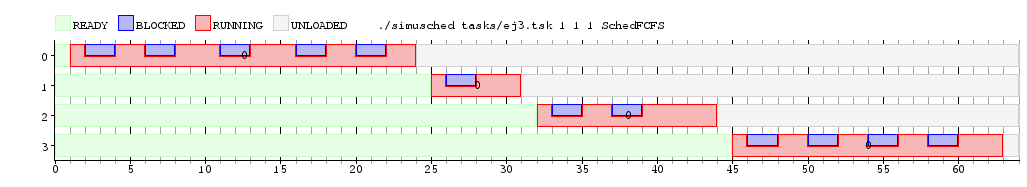
\includegraphics[width=1\columnwidth]{imagenes/ej3.png}
			\caption{Cuatro \texttt{TaskBatch} corriendo con el scheduler FCFS. $\texttt{total\_cpu}:13, 4, 8, 10$, $\texttt{cant\_bloqueos}:5, 1, 2, 4 $.}
		\end{center}
	\end{figure}


\section{Ejercicio 4}

En este ejercicio se pedía completar el scheduler round robin con única cola
global \texttt{SchedRR}. Para esto se tuvieron que programar las funciones que
requiere el simulador para utilizar un scheduler.

El constructor del scheduler toma como argumentos la cantidad de cores y el
quantum asociado a cada uno. Aquí lo único que se realizó fue cargar en un
vector el quantum asociado a cada core y duplicar el mismo para tener otro
donde poder modificar estos valores a medida que se van consumiendo.

\begin{codesnippet}
\begin{verbatim}
    def_quantum = Vector donde cada elemento es el quantum asociado a un núcleo
    cpu_quantum = Copia del vector anterior para llevar cuenta de los quantums consumidos
\end{verbatim}
\end{codesnippet}

La operación \texttt{load(int pid)} que es llamada cuando llega un proceso
nuevo, encola el proceso en la cola global del scheduler. La función
\texttt{unblock(int pid)} tiene el mismo comportamiento, dado que vuelve a
agregar una tarea que se encontraba bloqueada.

\begin{codesnippet}
\begin{verbatim}
load(pid)
    Encolar proceso pid a cola global
unblock(pid)
    Encolar proceso pid a cola global
\end{verbatim}
\end{codesnippet}

En \texttt{tick(int cpu, const enum Motivo m)} es donde se hace la gran parte
del trabajo, donde la acción a tomar depende del motivo del tick y el estado de
la cola:

\begin{codesnippet}
\begin{verbatim}
tick(cpu, motivo)
    Si la tarea corriendo en cpu es la idle
        Si la cola global no está vacía
            Desencolar el primero de la cola global y asignarlo a cpu
    Si no
        Si el motivo es TICK
            Decrementar el quantum en cpu_quantum[cpu]
            Si cpu_quantum[cpu] es 0
                Si la cola global no está vacía
                    Encolar proceso actual
                    Desencolar el primero de la cola global y asignarlo a cpu
                Si no
                    Dejar que siga corriendo el proceso actual
                Reiniciar quantum en cpu_quantum[cpu] con el valor dado por def_quantum[cpu]
            Si no
                Dejar que siga corriendo el proceso actual
        Si no, si el motivo es EXIT o BLOCK
            Si la cola global no está vacía
                Desencolar el primero de la cola global y asignarlo a cpu
            Reiniciar quantum en cpu_quantum[cpu] con el valor dado por def_quantum[cpu]
\end{verbatim}
\end{codesnippet}

Primero se consulta si la tarea del core actual es la idle, ya que
en caso de ser así es posible asignarle el mismo al primer proceso de la cola. Caso
contrario, se opera en base al motivo de la llamada.

Si llega con motivo \texttt{TICK}, se comienza decrementando en uno el quantum disponible
del núcleo actual. En el caso donde el quantum disponible llega a 0, si la cola
global está vacía se deja al proceso actual, caso contrario el mismo es
desalojado dándole lugar al siguiente en la cola. En ambas situaciones el
quantum es reiniciado a su valor inicial. Cuando el quantum aún no llegó a 0
simplemente se deja seguir ejecutando al proceso presente.

Si el motivo es \texttt{BLOCK} o \texttt{EXIT}, la tarea actual es desalojada
dándole lugar a la próxima en la cola con un quantum reiniciado.

\begin{figure}[ht]
	\begin{center}
		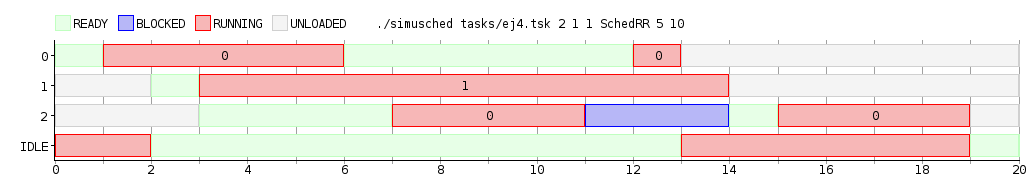
\includegraphics[width=1\columnwidth]{imagenes/ej4.png}
		\caption{\texttt{SchedRR} corriendo 3 tareas con dos núcleos: uno de 5 y
		otro de 10.}
	\end{center}
\end{figure}

\section{Ejercicio 5}
\label{sec:ej5}

Este ejercicio pedía experimentar con el scheduler round robin desarrollado en
el punto anterior. Para ello, primero se generó un lote con 3 tareas
\texttt{TaskCPU} de 70 ciclos y 2 \texttt{TaskConsola} con 3 llamadas
bloqueantes de duración 3. Luego se realizaron las siguientes pruebas donde lo
que se fue modificando fue la cantidad de núcleos y el quantum asignado a cada
uno.

En la Figura \ref{fig:ej1_3n} se configuró el simulador para utilzar 3 núcleos
con quantums de 2, 10 y 30. Se puede observar cómo al disponer de estos 3
núcleos las tareas se llevaron a cabo relativamente rápido dado que al disponer
de varios quantums los procesos pequeños pueden ejecutarse mientras que en
paralelo corren los más grandes.

\begin{figure}[H]
	\begin{center}
		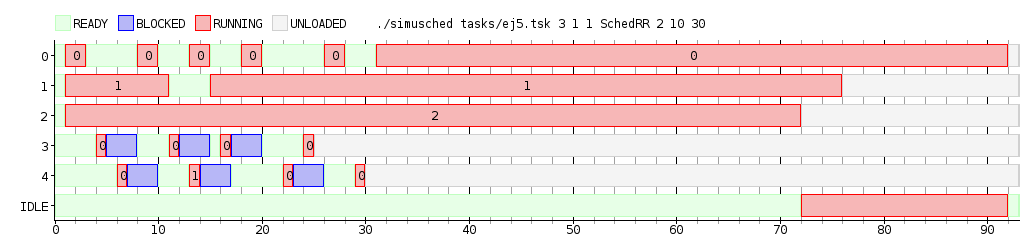
\includegraphics[width=1\columnwidth]{imagenes/ej5.png}
		\caption{\texttt{SchedRR} corriendo con tres núcleos: uno de quantum 2, 10 y otro de 30.}
		\label{fig:ej1_3n}
	\end{center}
\end{figure}

A continuación, se presentan los resultados de haber fijado la cantidad de núcleos
a 1 con un cambio de contexto de 2 ciclos variando únicamente el quantum para ver
así el efecto sobre la \emph{latencia}, \emph{waiting-time} y \emph{turnaround}
(tiempo total) promedio de las tareas descritas al comienzo del ejercicio.

\begin{figure}[H]
	\begin{center}
		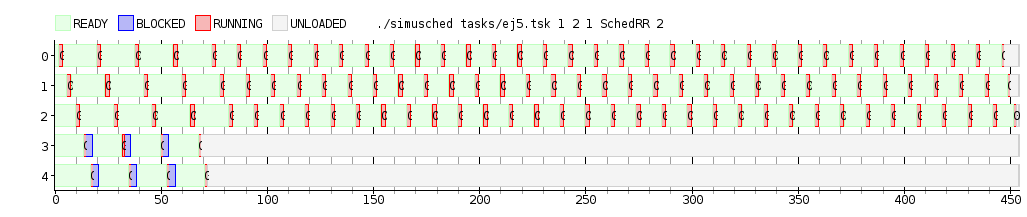
\includegraphics[width=1\columnwidth]{imagenes/ej5_q2.png}
		\caption{\texttt{SchedRR} corriendo con un núcleo de quantum 2}
	\end{center}
\end{figure}

\begin{figure}[H]
	\begin{center}
		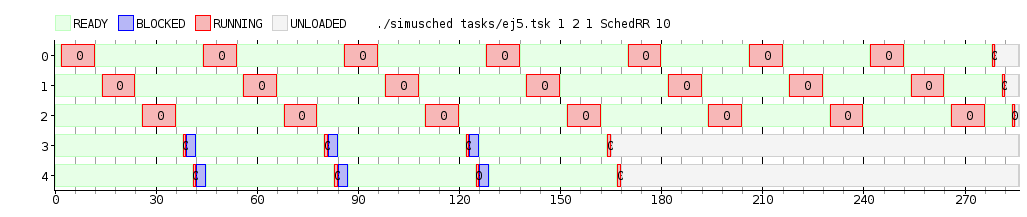
\includegraphics[width=1\columnwidth]{imagenes/ej5_q10.png}
		\caption{\texttt{SchedRR} corriendo con un núcleo de quantum 10}
	\end{center}
\end{figure}

\begin{figure}[H]
	\begin{center}
		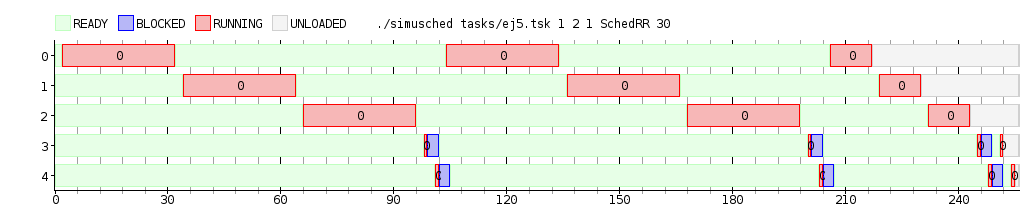
\includegraphics[width=1\columnwidth]{imagenes/ej5_q30.png}
		\caption{\texttt{SchedRR} corriendo con un núcleo de quantum 30}
	\end{center}
\end{figure}

Tomando los resultados anteriores se generó la siguiente tabla comparando los
tiempos para cada tamaño de quantum seleccionado.

\begin{table}[H]
	\begin{center}
		\begin{tabular}{|c|c|c|c|}
			\hline
			\textbf{Quantum} & \textbf{Latencia} & \textbf{Waiting-time} & \textbf{Turnaround} \\ \hline
			2 & 9,8 & 250,4 & 298,2 \\ \hline
			10 & 24,2 & 188 & 235,8 \\ \hline
			30 & 60,2 & 191,6 & 239,4 \\ \hline
		\end{tabular}
		\caption{Tiempos promedio en función del tamaño de quantum utilizado}
	\end{center}
\end{table}

A partir de esta información se pudieron desarrollar las siguiente conclusiones.
Para empezar, a simple vista se puede observar que ninguno de los tres tamaños
seleccionados es mejor en todos los criterios utilizados en simultáneo, esto
pone en evidencia el hecho de no existe una receta para todos los problemas, si
no que dependiendo las necesidades de uno, se debe decidir por alguno u otro.
Habiendo dicho esto, se pasan a describir los puntos fuertes y débiles de cada
quantum utilizado.

Para el quantum de \textbf{2}, la \emph{latencia} es la más baja con una amplia
diferencia respecto al resto. Esto es particularmente importante si se tienen
tareas interactivas donde se espera que el tiempo de respuesta sea alto. Sin
embargo, aquí se tiene que el \emph{waiting-time} y \emph{turnaround} son los
más altos de la tabla, indicando que en caso de tener tareas pesadas que
necesiten más tiempo del CPU este quantum no sería el apropiado.

Con un quantum de \textbf{10}, los resultados son bastante balanceados. La
\emph{latencia} es mejor que la del quantum de 30 pero peor que la de 2. Esto
tiene sentido ya que al aumentar el tamaño del quantum las tareas tienen que
esperar más a que termine su predecesor. Sin embargo, el \emph{waiting-time} es
el mejor de la tabla, y aquí es donde probablemente se deba a que con un quantum
de 10 se consigue el punto medio necesario para el lote de tareas generado, si
fuera muy pequeño, las tareas grandes desperdiciarían mucho tiempo
realizando cambio de contexto, si fuera grande, las tareas pequeñas deberían
esperar mucho para poder completarse.

Finalmente, fijando un quantum de \textbf{30}, se consiguen tiempos que son
ligeramente peores que los obtenidos por el de 10. En lo que es \emph{latencia},
es el peor de los tres, lo cual no es sorpresa ya que las primeras tareas en
ejecutarse son las de mayor consumo de CPU, dejando sin atender a las
bloqueantes. El \emph{waiting-time} es mejor que el de 2 pero levemente peor que
con 10, nuevamente debido al hecho de que al otrogarle más tiempo de
cómputo a las tareas intensivas, el resto espera más. Por último, el
\emph{turnaround}, que en principio uno podría suponer que sería el mejor (dado
que es el caso donde las tareas finalizan en menor tiempo) es también un
poco mayor que la de 10. Esto ocurre porque más allá de que finalicen antes que
el resto, el promedio es peor, ya que cuando se utilizaba un quantum de 10, las
tareas bloqueantes finalizaban antes.

Otro análisis posible es el de evaluar los valores de las métricas seleccionadas
para cada quantum en \texttt{TaskCPU} y \texttt{TaskConsola} por separado.

\begin{table}[H]
	\begin{center}
		\begin{tabular}{|c|c|c|c|c|}
			\hline
			\textbf{Quantum} & \textbf{Tipo tarea} & \textbf{Latencia} & \textbf{Waiting-time} & \textbf{Turnaround} \\ \hline
			\multirow{2}{*}{2} & \texttt{TaskCPU} & 6 & 373 & 444 \\ \cline{2-5}
			& \texttt{TaskConsola} & 15,5 & 42 & 55 \\ \hline \hline
			\multirow{2}{*}{10} & \texttt{TaskCPU} & 14 & 197 & 268 \\ \cline{2-5}
			& \texttt{TaskConsola} & 39,5 & 114 & 127 \\ \hline \hline
			\multirow{2}{*}{30} & \texttt{TaskCPU} & 34 & 125 & 196 \\ \cline{2-5}
			& \texttt{TaskConsola} & 99,5 & 141 & 154 \\ \hline
		\end{tabular}
		\caption{Tiempos promedio en función del tamaño de quantum utilizado y
		el tipo de tarea}
	\end{center}
\end{table}

Para la \emph{latencia}, tanto en \texttt{TaskCPU} como \texttt{TaskConsola} el
valor incrementa junto al tamaño del quantum. Por otro lado, el
\emph{waiting-time} al igual que el \emph{turnaround} disminuyen en
\texttt{TaskCPU} y aumentan en \texttt{TaskConsola}.

El aumento de \emph{latencia} en ambos es posible de explicar como resultado
inmediato de darle mayor quantum a cada proceso. Cada tarea tendrá que esperar
a que termine la anterior para poder comenzar, por lo tanto si están
recibiendo un mayor quantum es razonable que esta espera sea mayor.

Con respecto al \emph{waiting-time} y \emph{turnaround}, las tareas
\texttt{TaskConsola} consumen muy poco tiempo del CPU dado que se bloquean casi
instantáneamente, esto es favorecido por un quantum pequeño ya que son puestas
en ejecución con más frecuencia. Con las tareas \texttt{TaskCPU} la historia es
distinta, ya que no se bloquean nunca utilizando así todo el quantum que
disponen.

Dicho esto, que estas métricas aumenten para \texttt{TaskConsola}
tiene sentido ya que al bloquearse, hasta que no se ejecuten el resto de las tareas no
vuelve a correr, prolongando así el tiempo que se encuentra esperando y su tiempo
total de ejecución.

A su vez, que las métricas disminuyan con \texttt{TaskCPU} puede justificarse
con el hecho de que al ser una tarea que no se bloquea, requiere el mayor tiempo
en ejecución posible, puesto que al estar en espera no realiza ningún tipo de
progreso. Aumentando el quantum el proceso tiene más ciclos para trabajar sin
ser interrumpido logrando finalizar en menor tiempo y disminuyendo sus
intervalos de espera.

\section{Ejercicio 6}

Este punto busca mostrar las diferencias entre \emph{Round-Robin} y \emph{FCFS}.
Para ello, se ejecutó el mismo lote de tareas del ejercicio anterior utilizando
\texttt{SchedFCFS} como scheduler. La cantidad de núcleos se fijó en 1 y el
costo de cambio de contexto en 2.

\begin{figure}[H]
	\begin{center}
		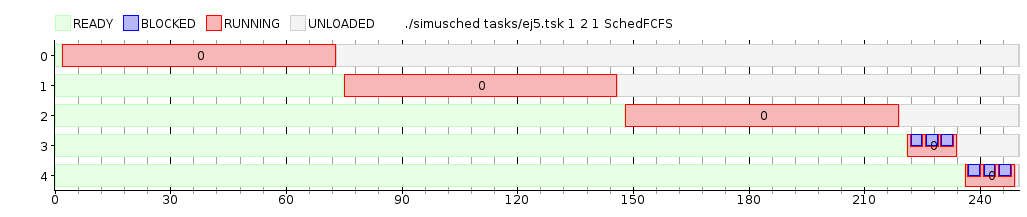
\includegraphics[width=1\columnwidth]{imagenes/ej6.png}
		\caption{\texttt{SchedFCFS} corriendo el lote de tareas del Ejercicio \ref{sec:ej5}}
	\end{center}
\end{figure}

Habiendo graficado el resultado de correr estas tareas con \texttt{SchedFCFS}
uno ya podría llegar a realizar algunas observaciones, pero con el objetivo de
tener más información a la hora de comparar, se calculó la
\emph{latencia}, \emph{waiting-time} y \emph{turnaround} promedio. Los valores
obtenidos se muestran a continuación.

\begin{table}[H]
	\begin{center}
		\begin{tabular}{|r|c|c|c|c|}
			\hline
			\textbf{Scheduler} & \textbf{Quantum} & \textbf{Latencia} & \textbf{Waiting-time} & \textbf{Turnaround} \\ \hline
			\texttt{SchedRR} & 2 & 9,8 & 250,4 & 298,2 \\ \cline{2-5}
			& 10 & 24,2 & 188 & 235,8 \\ \cline{2-5}
			& 30 & 60,2 & 191,6 & 239,4 \\ \hline
			\texttt{SchedFCFS} & N/A & 136,4 & 136,4 & 184,2 \\ \hline
		\end{tabular}
		\caption{Tiempos promedio en función del scheduler utilizado}
	\end{center}
\end{table}

Lo primero que llama la atención es la \emph{latencia}, ya que supera de forma
significativa la de las pruebas realizadas con \texttt{SchedRR}. Esto es fácil
de ver dado que cada tarea se corre de principio a fin, antes de cederle el
control a la siguiente. Claramente esta política no sería eficiente a la hora de
querer un sistema con procesos interactivos, ya que el tiempo de respuesta sería
enorme, dando al usuario la sensación de que el mismo dejó de funcionar por
completo.

Por otra parte, el \emph{waiting-time} tanto como el \emph{turnaround} dieron
valores más bajos. Esto se puede justificar con el hecho de que cualquier
implementación de \emph{Round-Robin} contará con el overhead de realizar cambios
de contextos sumado a que cada tarea tiene que esperar a que se de toda la
vuelta para ser asignada de nuevo.

Ahora, al analizarse con más cuidado es posible cuantificar estas diferencias para
poder pesarlas mejor en la balanza. Tomando el resultado de \texttt{SchedRR} con
quantum \textbf{10} y comparándolo contra el de \texttt{SchedFCFS} se tienen los
siguientes porcentajes asociados al último:

\begin{itemize}
	\item 463.6\% más de \emph{latencia}
	\item 37.8\% menos de \emph{waiting-time}
	\item 28\% menos de \emph{turnaround}
\end{itemize}

De aquí se puede apreciar cómo la mejoría en \emph{waiting-time} y
\emph{turnaround} es a cuestas de un gran deterioro en lo que es
\emph{latencia}.

Es por esto que se concluye que \emph{FCFS} tiene sentido cuando no interesa el
tiempo de respuesta y uno está dispuesto a sacrificar esa característica con tal
de obtener una mejoría en otros criterios como lo son el \emph{waiting-time} y
\emph{turnaround}.

\newpage
\section{Ejercicio 7}
	\subsection{Analisis del Schedler}

	Para entender el schedler, hemos corrido  una serie de tareas .

	\begin{figure}[ht]
		\begin{center}
			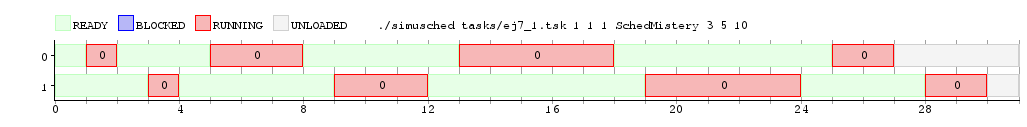
\includegraphics[width=1\columnwidth]{imagenes/ej7_1.png}
			\caption{Dos \texttt{TaskCPU} con 20 quantums.}
		\end{center}
	\end{figure}

	Se puede apreciar que cuando una  tarea acaba sus quantums, es quitada de la cola donde esta y es  agregada en la siguiente cola con menor prioridad , si es posible , en caso contrario quedara en la cola donde pertenece (La de menor prioridad) . Una vez que el schedler desencola todas las tareas pendientes en una cola pasa a la siguiente.


	\begin{figure}[ht]
		\begin{center}
			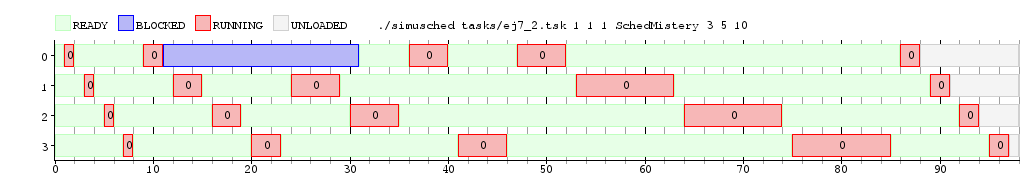
\includegraphics[width=1\columnwidth]{imagenes/ej7_2.png}
			\caption{Un \texttt{TaskCPU} corriendo con 20 quantums y tres \texttt{TaskAlterno} alterando 2 quantums de uso de kernel , 1 de bloqueo}
		\end{center}
	\end{figure}

	Como se puede apreciar este schedler permite starvation, es que las tareas con pocos ó ningun bloqueo se acumulen en las colas con menor prioridad, esperando ha que las tareas de mayor prioridad terminen para que les toque a ellas.
	Cuando una tarea se desbloquea , es la proxima tarea ha correr y su nivel de prioridad aumenta en uno.

	\begin{figure}[ht]
		\begin{center}
			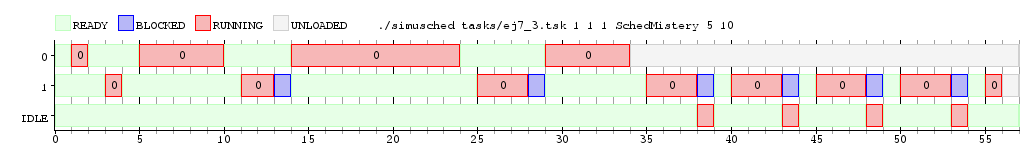
\includegraphics[width=1\columnwidth]{imagenes/ej7_3.png}
			\caption{Un \texttt{TaskCPU} corriendo con 20 quantums y un \texttt{TaskAlterno} alterando 2 quantums de uso de kernel , 1 de bloqueo al principio y despues 4 y 2.}
		\end{center}
	\end{figure}

	Como se ve la tarea IDEL  actua como se espera , cuando no hay nada para correr , corre la IDEL.

	Los quantums asignados a las colas de prioridad son 1 quatum a la de maxima prioridad y los argumentos pasados por parametro son las siguientes prioridades.

	\subsection{Implementación del Schedler}




\section{Ejercicio 8}

Se pedía implementar un scheduler, \texttt{SchedRR2}, con modalidad Round-Robin
y que no permitiera migrar los procesos entre núcleos. El CPU correspondiente a
cada proceso es seleccionado durante su carga, correspondiendo en cada caso
aquel con menor cantidad total de procesos activos.

\subsection{Implementación del scheduler}

Al igual que en ejercicios anteriores, el constructor del scheduler recibe por
parámetro la cantidad de cores y el tiempo del \emph{quantum} correspondiente a
cada uno de ellos. Estos valores son almacenados, guardando por duplicado la
duración de los \emph{quantums} para luego poder ir decrementando una de las
copias. Durante la inicialización, además, se crean estas estructuras
adicionales: un vector para almacenar la cantidad de procesos que se están
ejecutando en cada procesador, un vector de vectores que contiene los PIDs de
cada uno de ellos, y un vector con las colas de \emph{ready} correspondientes a
cada \emph{core}.

Al cargar un proceso en el scheduler, se utiliza el primero de los vectores
mencionados para seleccionar el núcleo que tenga menos procesos activos. Luego
el proceso recién cargado se agrega en la cola de \emph{ready} del core y en su
lista de tareas activas, y se incrementa en uno su contador de procesos.

Cuando se produce una llamada a la función \texttt{tick}, es decir, cuando se
produce un \emph{tick} del reloj de algún CPU y el \emph{scheduler} es invocado,
se realizan diferentes acciones según cuál haya sido la actividad de la CPU
durante el \emph{quantum} anterior.

En varias ocasiones se relizan llamadas a la función auxiliar \texttt{next}, que
desencola la próxima tarea de la cola de \emph{ready} de una CPU y devuelve su
PID, en caso de que esto sea posible, y en caso contrario devuelve el PID de la
tarea \emph{idle}. Además, esta función reinicia el contador de tiempo de
\emph{quantum} restante del CPU a su valor inicial.

\begin{enumerate}
    \item Si el proceso anterior consumió todo el ciclo de CPU, puede tratarse
    de la tarea \emph{idle}, en cuyo caso simplemente se realiza una llamada a
    \texttt{next}, o bien puede tratarse de otra tarea en ejecución. En este
    caso se chequea si aún sobra tiempo del \emph{quantum} actual. De ser así,
    se decrementa en uno el contador de tiempo restante y se decide que siga
    ejecutando el mismo proceso. En caso contrario, se desaloja al proceso
    utilizando la función \texttt{next} y se lo vuelve a colocar en la cola de
    \emph{ready}.
    \item Si el proceso anterior realizó una llamada bloqueante, simplemente se
    lo desaloja con la función \texttt{next}. Cuando el proceso se desbloquee,
    la función \texttt{unblock} se encargará de hacerlo volver a la cola de
    \emph{ready}.
    \item Si el proceso anterior acaba de terminar, entonces se lo reemplaza por
    el proceso siguiente ejecutando \texttt{next} y, además, se lo elimina de
    las lista de tareas activas del CPU donde estaba registrado. También se
    decrementa en uno el contador de tareas activas de este CPU.
\end{enumerate}

\subsection{Experimentación}

Se pedía realizar una comparación entre este criterio de \emph{scheduling}
y otro que sí permitiera la migración entre procesadores. Con este fin, se
comparó el \emph{scheduler} obtenido con el desarrollado anteriormente en el
Ejercicio 4 (\texttt{SchedRR}).

Para comparar los resultados producidos por ambos \emph{schedulers}, se
plantearon dos ejemplos de escenarios reales en los que cada uno de los modelos
resultara superior al otro. Los escenarios ideados fueron los siguientes:

\begin{enumerate}
    \item En una máquina con dos CPUs y un coste de migración apreciable, se
    ejecutan simultáneamente tres tareas que hacen un uso intensivo del
    procesador. Además, los tiempos de \emph{quantum} asociados a cada
    procesador son diferentes. En estas circunstancias, es esperable que un
    scheduler con migración produzca que los procesos estén cambiando de CPU de
    manera constante, generando un gran desperdicio de recursos. Este efecto
    seguramente afecte negativamente métricas como el \emph{waiting-time} y el
    \emph{turnaround} de los procesos, lo cual es indeseable en este tipo de
    tareas no interactivas. Cabe destacar que en el caso del \emph{scheduler}
    \texttt{SchedRR2} uno de los procesos tendrá un CPU asignado de forma
    exclusiva, mientras que los otros dos tendrán que ``repartirse'' el otro
    \emph{core}, reduciendo la \emph{justicia} del algoritmo. No obstante,
    teniendo en cuenta lo antes planteado, en este contexto es claramente
    preferible un algoritmo de \emph{scheduling} sin migración.

    \item También en una máquina con dos CPUs, se ejecuta una tarea que hace un
    uso intensivo del CPU y varias tareas interactivas, es
    decir, que hacen un gran uso de entrada/salida. Aquí el \emph{scheduler} sin
    migración asignará a la mitad de las tareas interactivas el mismo
    \emph{core} que a la tarea intensiva, provocando una disminución en la 
    \emph{latencia} o tiempo de respuesta de las mismas, como así también en su
    tiempo de espera o \emph{waiting-time}. El \emph{scheduler} con migración,
    en cambio, permitirá que, mientras la tarea intesiva utiliza un procesador, 
    cualquiera de las tareas interactivas pueda ocupar el otro, obteniendo así
    mejores resultados.
\end{enumerate}

A continuación se muestran los gráficos y las mediciones obtenidas en ambas
implementaciones para los lotes de tareas \texttt{ej8\_1} y \texttt{ej8\_2},
realizados según los dos escenarios recién propuestos.

\begin{figure}[H]
    \begin{center}
        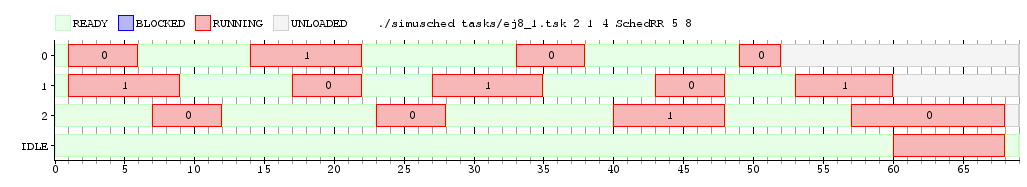
\includegraphics[width=1\columnwidth]{imagenes/ej8_1_rr.png}
        \caption{Escenario 1 en \emph{scheduler} con migración (\texttt{SchedRR})}
    \end{center}
\end{figure}

\begin{figure}[H]
    \begin{center}
        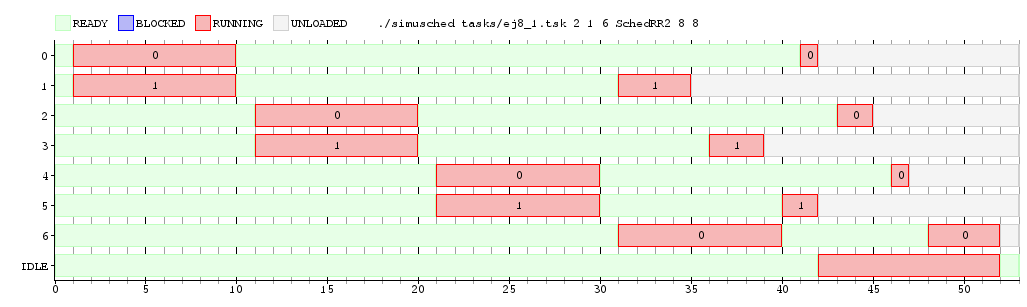
\includegraphics[width=1\columnwidth]{imagenes/ej8_1_rr2.png}
        \caption{Escenario 1 en \emph{scheduler} sin migración (\texttt{SchedRR2})}
    \end{center}
\end{figure}

\begin{figure}[H]
    \begin{center}
        \begin{tabular}{|c|c|c|c|}
            \hline
            \textbf{Scheduler} & \textbf{Waiting-time} & \textbf{Turnaround} \\ \hline
            \texttt{SchedRR}   & 32.333 & 60 \\
            \texttt{SchedRR2}  & 18.333 & 46 \\ \hline
        \end{tabular}
        \caption{Tiempos promedio para el Escenario 1, para cada \emph{scheduler}}
    \end{center}
\end{figure}


\begin{figure}[H]
    \begin{center}
        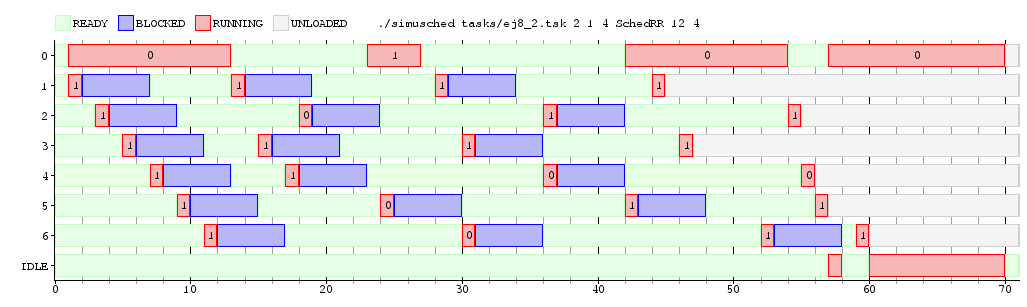
\includegraphics[width=1\columnwidth]{imagenes/ej8_2_rr.png}
        \caption{Escenario 2 en \emph{scheduler} con migración (\texttt{SchedRR})}
    \end{center}
\end{figure}

\begin{figure}[H]
    \begin{center}
        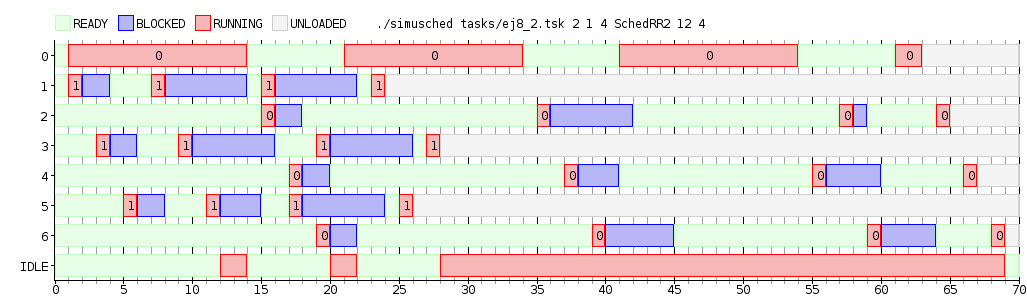
\includegraphics[width=1\columnwidth]{imagenes/ej8_2_rr2.png}
        \caption{Escenario 2 en \emph{scheduler} sin migración (\texttt{SchedRR2})}
    \end{center}
\end{figure}

\begin{figure}[H]
    \begin{center}
        \begin{tabular}{|c|c|c|c|}
            \hline
            \textbf{Scheduler} & \textbf{Latencia} & \textbf{Waiting-time} \\ \hline
            \texttt{SchedRR}   & 5.286 &  \\
            \texttt{SchedRR2}  & 8.714 &  \\ \hline
        \end{tabular}
        \caption{Tiempos promedio para el Escenario 2, para cada \emph{scheduler}}
    \end{center}
\end{figure}


\end{document}
